\vspace{0.5cm}
´

\begin{minipage}{0.99\linewidth}

\exo

Calculer la longueur manquante (si nécessaire, l'arrondir au millimètre près).

\begin{center}{3}
~\\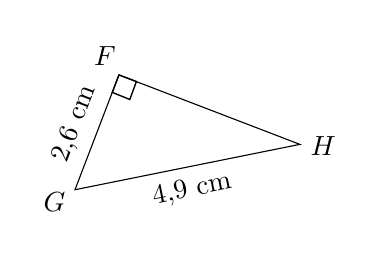
\begin{tikzpicture}[baseline,scale = 0.6]

    \tikzset{
      point/.style={
        thick,
        draw,
        cross out,
        inner sep=0pt,
        minimum width=5pt,
        minimum height=5pt,
      },
    }
    \clip (-1.9317566688177819,-3.4273091088927243) rectangle (4.827679748638527,1);


    	\draw[color={black},line width = 0.5] (0,0)--(-0.14,-0.37)--(0.23,-0.52)--(0.37,-0.14)--cycle;
	\draw[color={black}] (0,0)--(-0.93,-2.43)--(3.83,-1.47)--cycle;
	
	\draw [color={black}] (-0.298247790663296,0.401308180036817) node[anchor = center,scale=1] {$F$};
	\draw [color={black}] (-1.3614795963451893,-2.682922499694683) node[anchor = center,scale=1] {$G$};
	\draw [color={black}] (4.326795737602228,-1.4990277714686935) node[anchor = center,scale=1] {$H$};
	\draw [color={black}] (-0.93,-1.03) node[anchor = center, rotate = 69] {2,6 cm};
	\draw [color={black}] (1.55,-2.44) node[anchor = center, rotate = -348.62] {4,9 cm};

\end{tikzpicture}
\end{center}


\exo

Le triangle $NOP$ est tel que $NO=81$ cm, $NP=80$ cm et $OP=18$ cm.\\


1) Faire un croquis à main levée et y coder les informations du texte. \\

2) Ce triangle est-il rectangle ? Justifiez votre réponse. \\


\end{minipage}


